% !TeX program = xelatex
\documentclass[11pt,a4paper]{ctexart}
\usepackage[margin=2.2cm]{geometry}
\usepackage{amsmath,amssymb,booktabs,tabularx,array,graphicx,enumitem,xcolor,hyperref,float}
\hypersetup{colorlinks=true,linkcolor=black,urlcolor=blue}
\setlength{\parskip}{0.45em}\setlength{\parindent}{0pt}
\renewcommand{\arraystretch}{1.25}
\setlist{nosep,leftmargin=1.8em}
\graphicspath{{../../Figures/v7/}}
\newcolumntype{L}{>{\raggedright\arraybackslash}X}
\newcolumntype{P}[1]{>{\raggedright\arraybackslash}p{#1}}
\title{基于 v7 数据的模型一：植被—水—沙动力学\\[2pt]\large 重建版，2026-11-10}
\author{2026 CQU\_MCM B题 任务一}
\date{}
\begin{document}
\maketitle

\noindent\textbf{这是什么。}在 v7 数据面板上重建的模型一。它原样保留 \texttt{Reports/model\_v7.tex} 的年尺度状态方程，只增加一条水量关系，并且只拟合数据能够识别的两个参数。所有数字由 \texttt{Code/v7\_model1.py} 计算，保存在 \texttt{Results/v7/model1/}；详细证据见 \texttt{Docs/20261110\_model1\_v7\_rebuild.md}。图中文字为英文。

\section{模型}
\textbf{植被}（v7 方程，年步长；$V$ 为覆盖度 \%，v7 口径）：
\begin{equation}
V_{t+1}=V_t+\underbrace{r\,V_t\Bigl(1-\frac{V_t}{K}\Bigr)W_t}_{\text{生长}}-\underbrace{d\,V_t}_{\text{衰亡}}-\underbrace{k\,E_t\Bigl(1-\eta\frac{V_t}{K}\Bigr)V_t}_{\text{风蚀}} .
\end{equation}
\textbf{有效土壤水分}（新增关系）：
\begin{equation}
W_t=\min\Bigl\{1,\ \frac{A_t}{c\,\min(1,2f_{c,t})\,\mathrm{ET}_{0g}}\Bigr\},\qquad
A_t=\eta_w I_t+G,\qquad f_{c,t}=\frac{V_t}{V_{\mathrm{full}}} .
\end{equation}
$W$ 是植物可用水量与冠层不受胁迫时蒸腾需水量之比。$I$ 为毛灌溉量（mm/年），$G$ 为地下水补给，$\mathrm{ET}_{0g}=\sum_m f(T_m)\,\mathrm{ET}_{0,m}$ 为按温度加权的参考蒸散，$f_c$ 为地面覆盖比例。根区储水量（约 75 mm）远小于每年数百毫米的水通量，因此在年尺度上水分由供需决定，不需要单独的储水方程。

\textbf{耦合关系。}水 $\to$ 植被：$W$ 调节生长。植被 $\to$ 水：覆盖度越高需水越多，$W$ 越低。植被 $\to$ 沙：遮蔽因子 $(1-\eta V/K)$。沙 $\to$ 植被：风蚀项。

\textbf{稳态。}给定 $W$ 时 v7 的解析式仍然成立：
\begin{equation}
x^*=\frac{V^*}{K}=\frac{rW-d-kE}{rW-kE\eta},\qquad\text{当 }W=1,\ k=0\text{ 时：}\quad x^*=1-\frac{d}{r}=0.80 .
\end{equation}

\begin{table}[H]\small
\begin{tabularx}{\linewidth}{@{}P{2.2cm}P{5.4cm}L@{}}
\toprule
参数 & 取值 & 状态\\
\midrule
$r$ & $0.584\pm0.180$ 年$^{-1}$ & 拟合，7 个站点合并\\
$d$ & $0.117\pm0.035$ 年$^{-1}$ & 拟合，7 个站点合并\\
$K$ & 训练期 $V$ 的 95\% 分位 $\times1.15$，逐站确定；区段为 38.1\% & v7 规则，未改\\
$k$ & 0（估计值 $0.00\pm0.27$） & 不可识别；情景范围 0--0.10\\
$\eta$ & 1 & 固定；不可识别\\
$c$ & 1.0 & 假设，范围 0.7--1.2（FAO-56）\\
$\eta_w$ & 0.75 & 假设，范围 0.65--0.85\\
$V_{\mathrm{full}}$ & 66.6\%（v7 口径） & 取自区段内绿洲像元\\
$\mathrm{ET}_{0g}$ & 1163 mm/年 & v7 面板，于田、民丰站\\
\bottomrule
\end{tabularx}
\end{table}

\section{数据}
\begin{table}[H]\small
\begin{tabularx}{\linewidth}{@{}P{4.5cm}P{5.2cm}L@{}}
\toprule
数据 & 来源 & 用途\\
\midrule
v7 月尺度面板，9 站，2015--2025 & NASA POWER、MODIS MOD13Q1、ERA5（\texttt{Data/v7/processed/}） & 年值 $V$、$E$、ET$_0$；拟合 $r$、$d$\\
217 个由裸沙变为植被的像元，2003--2021 & 于田—民丰南缘 MODIS MOD13Q1（\texttt{Data/v7/section\_modis/}） & 独立检验 $r$、$d$\\
\bottomrule
\end{tabularx}
\end{table}
年值 $V$ 取 6--9 月有实际观测月份的平均。7 个站点有植被（于田、民丰、且末、若羌、库尔勒、尉犁、阿拉尔）；肖塘、塔中为沙漠。目标年份在 2022 年及以前的用于拟合，2023--2025 年留出检验。

\section{对 v7 的复核与修改}
\begin{table}[H]\small
\begin{tabularx}{\linewidth}{@{}P{0.5cm}P{3.8cm}P{5.6cm}L@{}}
\toprule
 & 发现 & 证据 & 修改\\
\midrule
C1 & 逐站用 8 个年值拟合 4 个参数不可行 & v7 消融表：训练 $R^2$ 中位数 0.004；89\% 的拟合顶到边界 & 所有有植被站点共用一组参数，$K$ 逐站\\
C2 & $k$、$\eta$ 无法估计 & 加入 $k$：AIC 由 $-282.4$ 变为 $-280.4$，$k=0.00\pm0.27$；加入 $\eta$：条件数 $2.6\times10^{8}$ & 只保留 $(r,d)$；$k$、$\eta$ 作为情景参数\\
C3 & v7 的水分指标（GWETROOT 归一化）没有时间信号 & 99.94\% 的方差来自站点之间；站内年际标准差 0.003--0.013；再分析不含灌溉 & $W$ 由水量关系给出；拟合时灌溉绿洲站点取 $W=1$\\
C4 & 年尺度上 $f(T)$ 与 $r$ 无法区分 & 站内年均气温变幅不超过 1.8\,$^\circ$C & $f(T)$ 并入 $r$，并保留在 ET$_{0g}$ 中\\
C5 & 插补的 NDVI 月份被当作观测评分 & 9.3\% 的站—月为插补，库尔勒 31\% & 年值 $V$ 只用实际观测月份\\
C6 & 固定端元 0.05/0.85 低估地面覆盖 & 最密的绿洲像元 NDVI 为 0.583，即 v7 口径下 66.6\% & 需要地面覆盖比例时除以 $V_{\mathrm{full}}$\\
C7 & 任务二使用的 $K_s=0.45+0.55\,I/60$ 没有依据 & \texttt{v7\_ablation.py} & 改用第 5 节的曲线\\
\bottomrule
\end{tabularx}
\end{table}

\section{数据支持}
\begin{table}[H]\small\centering
\begin{tabular}{@{}lccc@{}}
\toprule
站点，提前一年预测（$V/K$） & 训练 RMSE & 留出 RMSE & 留出 $R^2$\\
\midrule
模型 $(r,d)$ & 0.054 & 0.068 & 0.40\\
持续性基线（明年等于今年） & 0.060 & 0.058 & --\\
站点均值 & -- & 0.079 & --\\
\bottomrule
\end{tabular}
\end{table}
在留出年份上，模型优于站点均值，但不如持续性基线。站点序列都在稳态附近，只能确定比值 $d/r$ 和松弛速率，信息有限。

\begin{table}[H]\small\centering
\begin{tabular}{@{}lcc@{}}
\toprule
区段像元（$R^2$） & CON1--3（拟合 $K$、$V_0$） & CON4（从未使用）\\
\midrule
站点的 $r$、$d$ 直接迁移，不重新拟合 & 0.40 & 0.31\\
四个参数全部自由拟合 & 0.40 & 0.29\\
均值基线 & 0.00 & $-0.02$\\
\bottomrule
\end{tabular}
\end{table}
对这些像元自由拟合得到 $r=0.64$、$d=0.10$，站点结果为 $0.58$ 和 $0.12$。两套数据的地点、年份和动态过程都不同，结果却一致，这是 $r$、$d$ 最主要的数据支持。

\begin{figure}[H]\centering
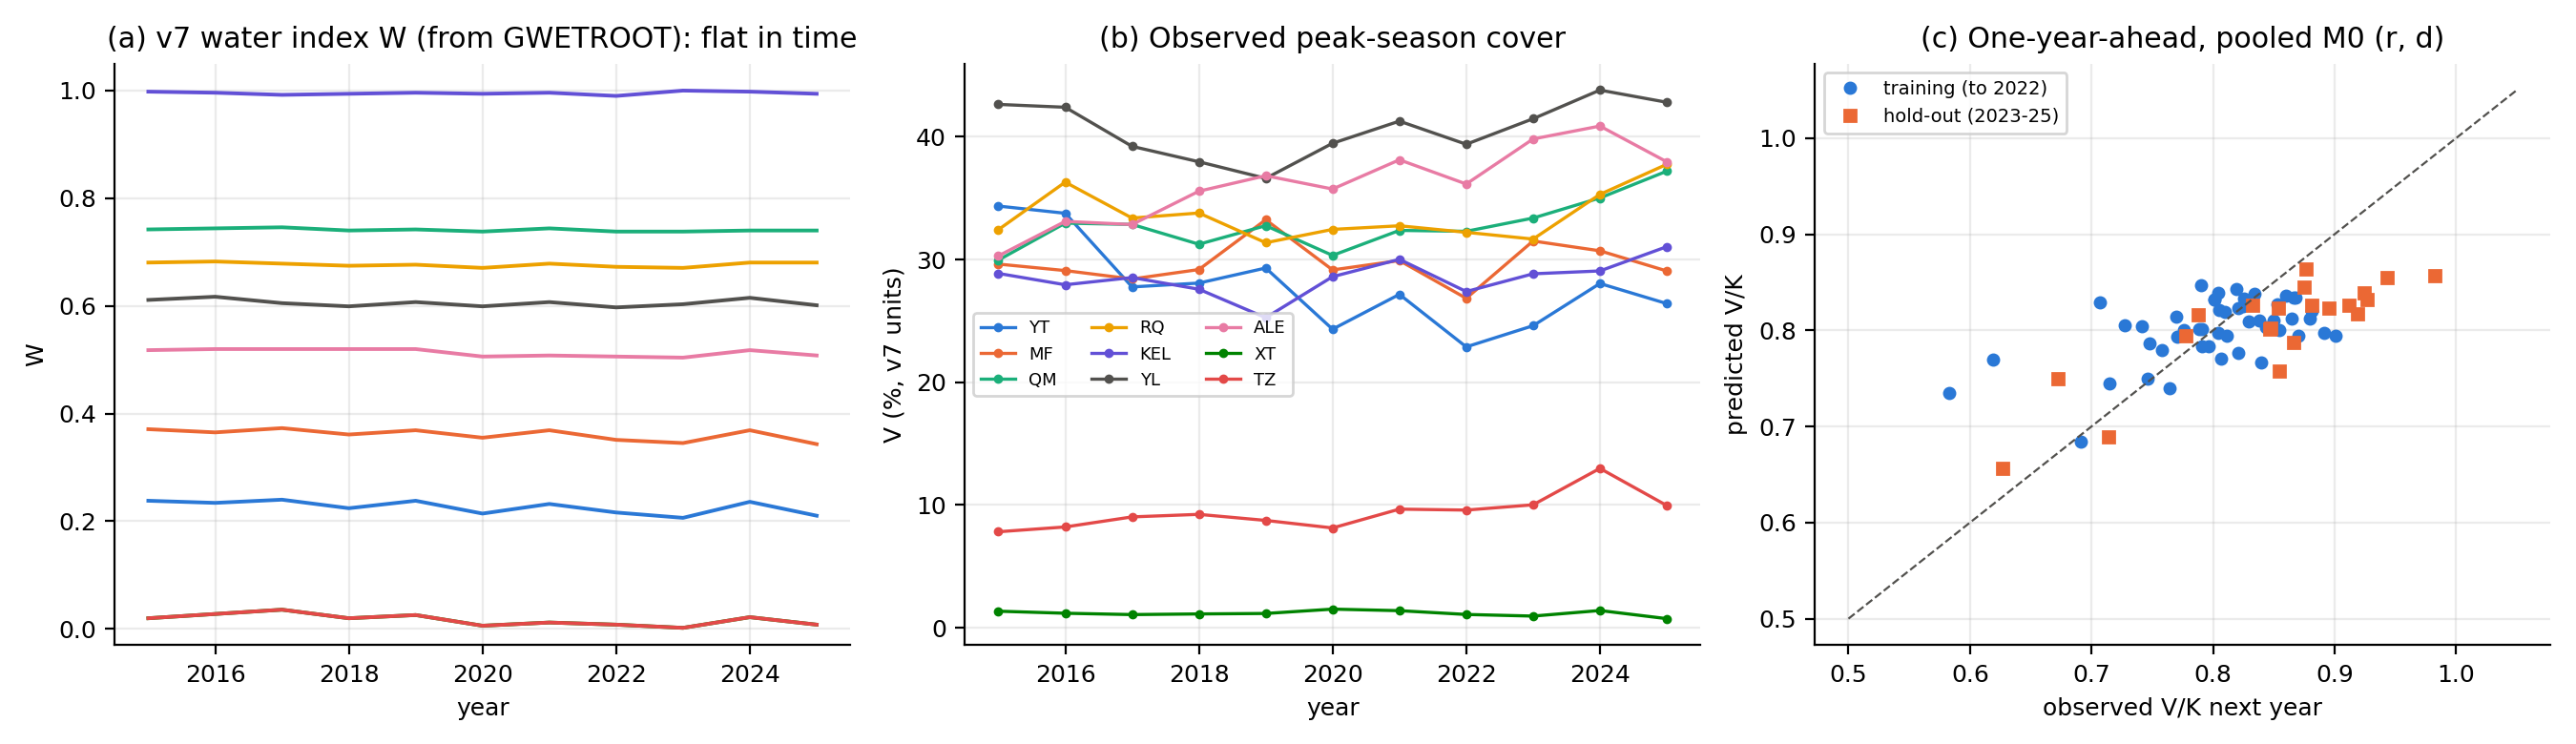
\includegraphics[width=\linewidth]{m1_fig1_station_evidence.png}
\caption{(a) v7 水分指标随时间几乎不变。(b) 观测的生长季覆盖度。(c) 合并模型的提前一年预测。}
\end{figure}

\section{结果}
\begin{table}[H]\small\centering
\begin{tabular}{@{}lrrrrrrrr@{}}
\toprule
毛灌溉量（mm/年） & 0 & 100 & 200 & 300 & 400 & 600 & 800 & 1000\\
\midrule
稳态 $V$（\%，v7 口径） & 0 & 8.3 & 13.7 & 17.4 & 20.1 & 23.9 & 26.3 & 28.1\\
地面覆盖比例 & 0 & 0.13 & 0.21 & 0.26 & 0.30 & 0.36 & 0.40 & 0.42\\
$W$ & 0 & 0.26 & 0.31 & 0.37 & 0.43 & 0.54 & 0.65 & 0.77\\
相对裸沙的风蚀强度 & 1.00 & 0.78 & 0.64 & 0.54 & 0.47 & 0.37 & 0.31 & 0.26\\
\bottomrule
\end{tabular}
\end{table}
\begin{itemize}
\item 1 mm/年相当于 10 m$^3$/ha/年。约 1420 mm/年以上水分不再是限制因素。
\item 新植林 10--11 年达到稳态覆盖度的 90\%。
\item 仅靠降水：覆盖度趋于零（肖塘站 1.2\%；区段沙漠像元 0.2\%）。
\item 天然过渡带（v7 口径 8.9\%）对应约 81 mm/年的地下水补给。
\item 300 mm/年下的稳态覆盖度在各敏感性情形中为 14--21\%；影响最大的是 $r$、$d$ 和 $c$。
\end{itemize}
\begin{figure}[H]\centering
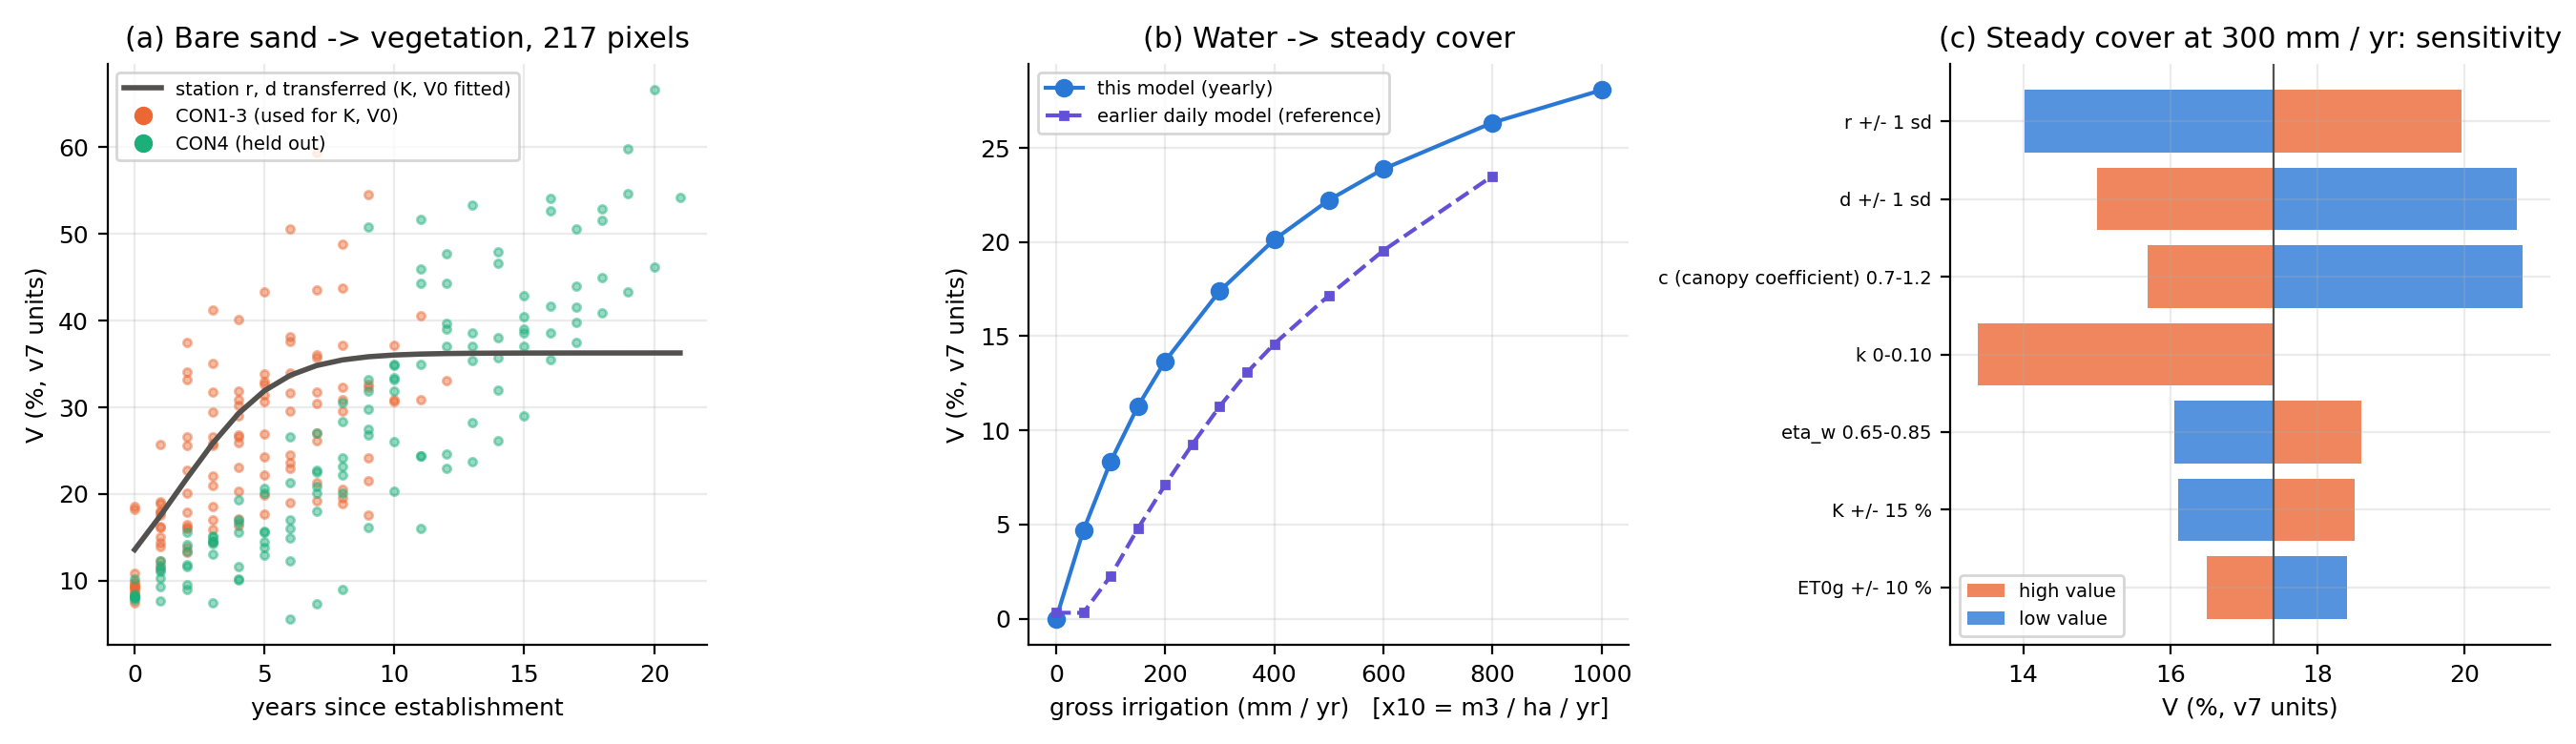
\includegraphics[width=\linewidth]{m1_fig2_transfer_and_water.png}
\caption{(a) 站点参数迁移到“裸沙变植被”像元。(b) 灌水量—稳态覆盖度，并以早先的日尺度模型作参照。(c) 300 mm/年下稳态覆盖度的敏感性。}
\end{figure}

\section{局限}
\begin{enumerate}
\item 站点覆盖度的提前一年预测不优于持续性基线。
\item 曲线的水分受限区间没有实测数据支撑，取决于假设的 $c$ 和 $\eta_w$。
\item 停止灌溉后，模型只按 $d$ 衰减（半衰期 5.9 年）。$d$ 是在有水的植被上得到的，实际损失很可能更快；任务三应把它当作情景处理。
\item $k$ 不可识别；风在任务三中只能作为情景。
\item 站点是绿洲内的城镇坐标，反映的是灌溉条件下的绿洲边缘植被，而不是沙丘上的灌木林带。
\end{enumerate}
\end{document}
